\documentclass[12pt,a4paper]{article}

\usepackage[margin=1in]{geometry}
\usepackage{microtype}
\usepackage{parskip}
\usepackage{graphicx}
\usepackage{hyperref}
\usepackage{setspace}
\usepackage{booktabs}  % for nicer tables

\doublespacing

\title{\Huge\bfseries 379k Final Report}
%\author{}
\date{\today}

\begin{document}
\maketitle

\section{Team Members}

\begin{itemize}
    \item Maanav Koladia
    \item Karemeldin Mohamed
    \item Andres Wearden
    \item Shrikar Thangavel
\end{itemize}

\section{Team Roles and Responsibilities}
All team members contributed collectively to every stage of the project, including design, implementation, testing, and documentation. Rather than assigning fixed roles, responsibilities were distributed dynamically based on project requirements and individual expertise. This collaborative approach ensured that all members gained experience across the full development cycle and that the project benefited from diverse perspectives and skill sets.

\section{Executive Summary}

This project's goal was to create a high-performance, real-time 2D fluid simulator that was both visually realistic and numerically stable. The core problem addressed was simulating an incompressible fluid (like water) in a way that conserved mass—preventing it from “squishing” or “expanding”—while running at interactive frame rates. The overall approach was a decoupled, three-service architecture built in C. First, a physics service (FS-2D) used CUDA on the GPU to perform the heavy computational work of solving the fluid dynamics equations on a 2D grid. Second, a Transform service, parallelized across a CPU thread pool, consumed this physics data and converted the fluid’s 2D state (an implicit level-set grid) into an explicit polygonal mesh using a marching-squares–style isocontouring algorithm.

This generated mesh was then passed to an independent GL/Display service, which used OpenGL to render the fluid with appropriate shading. By decoupling these stages with multi-threaded Lock-Free FIFO queues, the system avoided bottlenecks and allowed the physics simulation to run at a fixed, stable 60 steps per second independent of the final render frame rate. The intended outcome was a stable, interactive live demo of a 2D water simulation achieving 20–30 FPS, with an architecture designed to be directly scalable to future 3D extensions.

\section{System Design}

The entire system operates within a producer-consumer model implemented through three long-lived threads. The simulation thread advances the fluid state by running the Navier–Stokes solver at a fixed timestep. After completing each update, it packages the grid state into a snapshot and pushes this structure into a lock-free queue.

The transform thread continuously polls the simulation queue. When a snapshot becomes available, the transform thread converts the staggered grid data into a render frame. This conversion includes flattening the velocity and pressure fields, mapping simulation coordinates to pixel coordinates, and preparing buffers for eventual GPU transfer. After processing the snapshot, the transform thread pushes the completed frame into a second lock-free queue for consumption by the renderer.

The render thread owns the OpenGL context. It operates independently of the other threads and continuously retrieves the most recent frame from the transform queue. It then draws the data to the display or exports the frame to storage. Since these three threads do not block each other, the simulation can progress even if rendering becomes expensive, and the renderer can continue drawing even if the numerical solver slows down due to increased computational load. This decoupled structure preserves smooth visual output and stable physics stepping.

\begin{figure}[h] % h = here
    \centering
    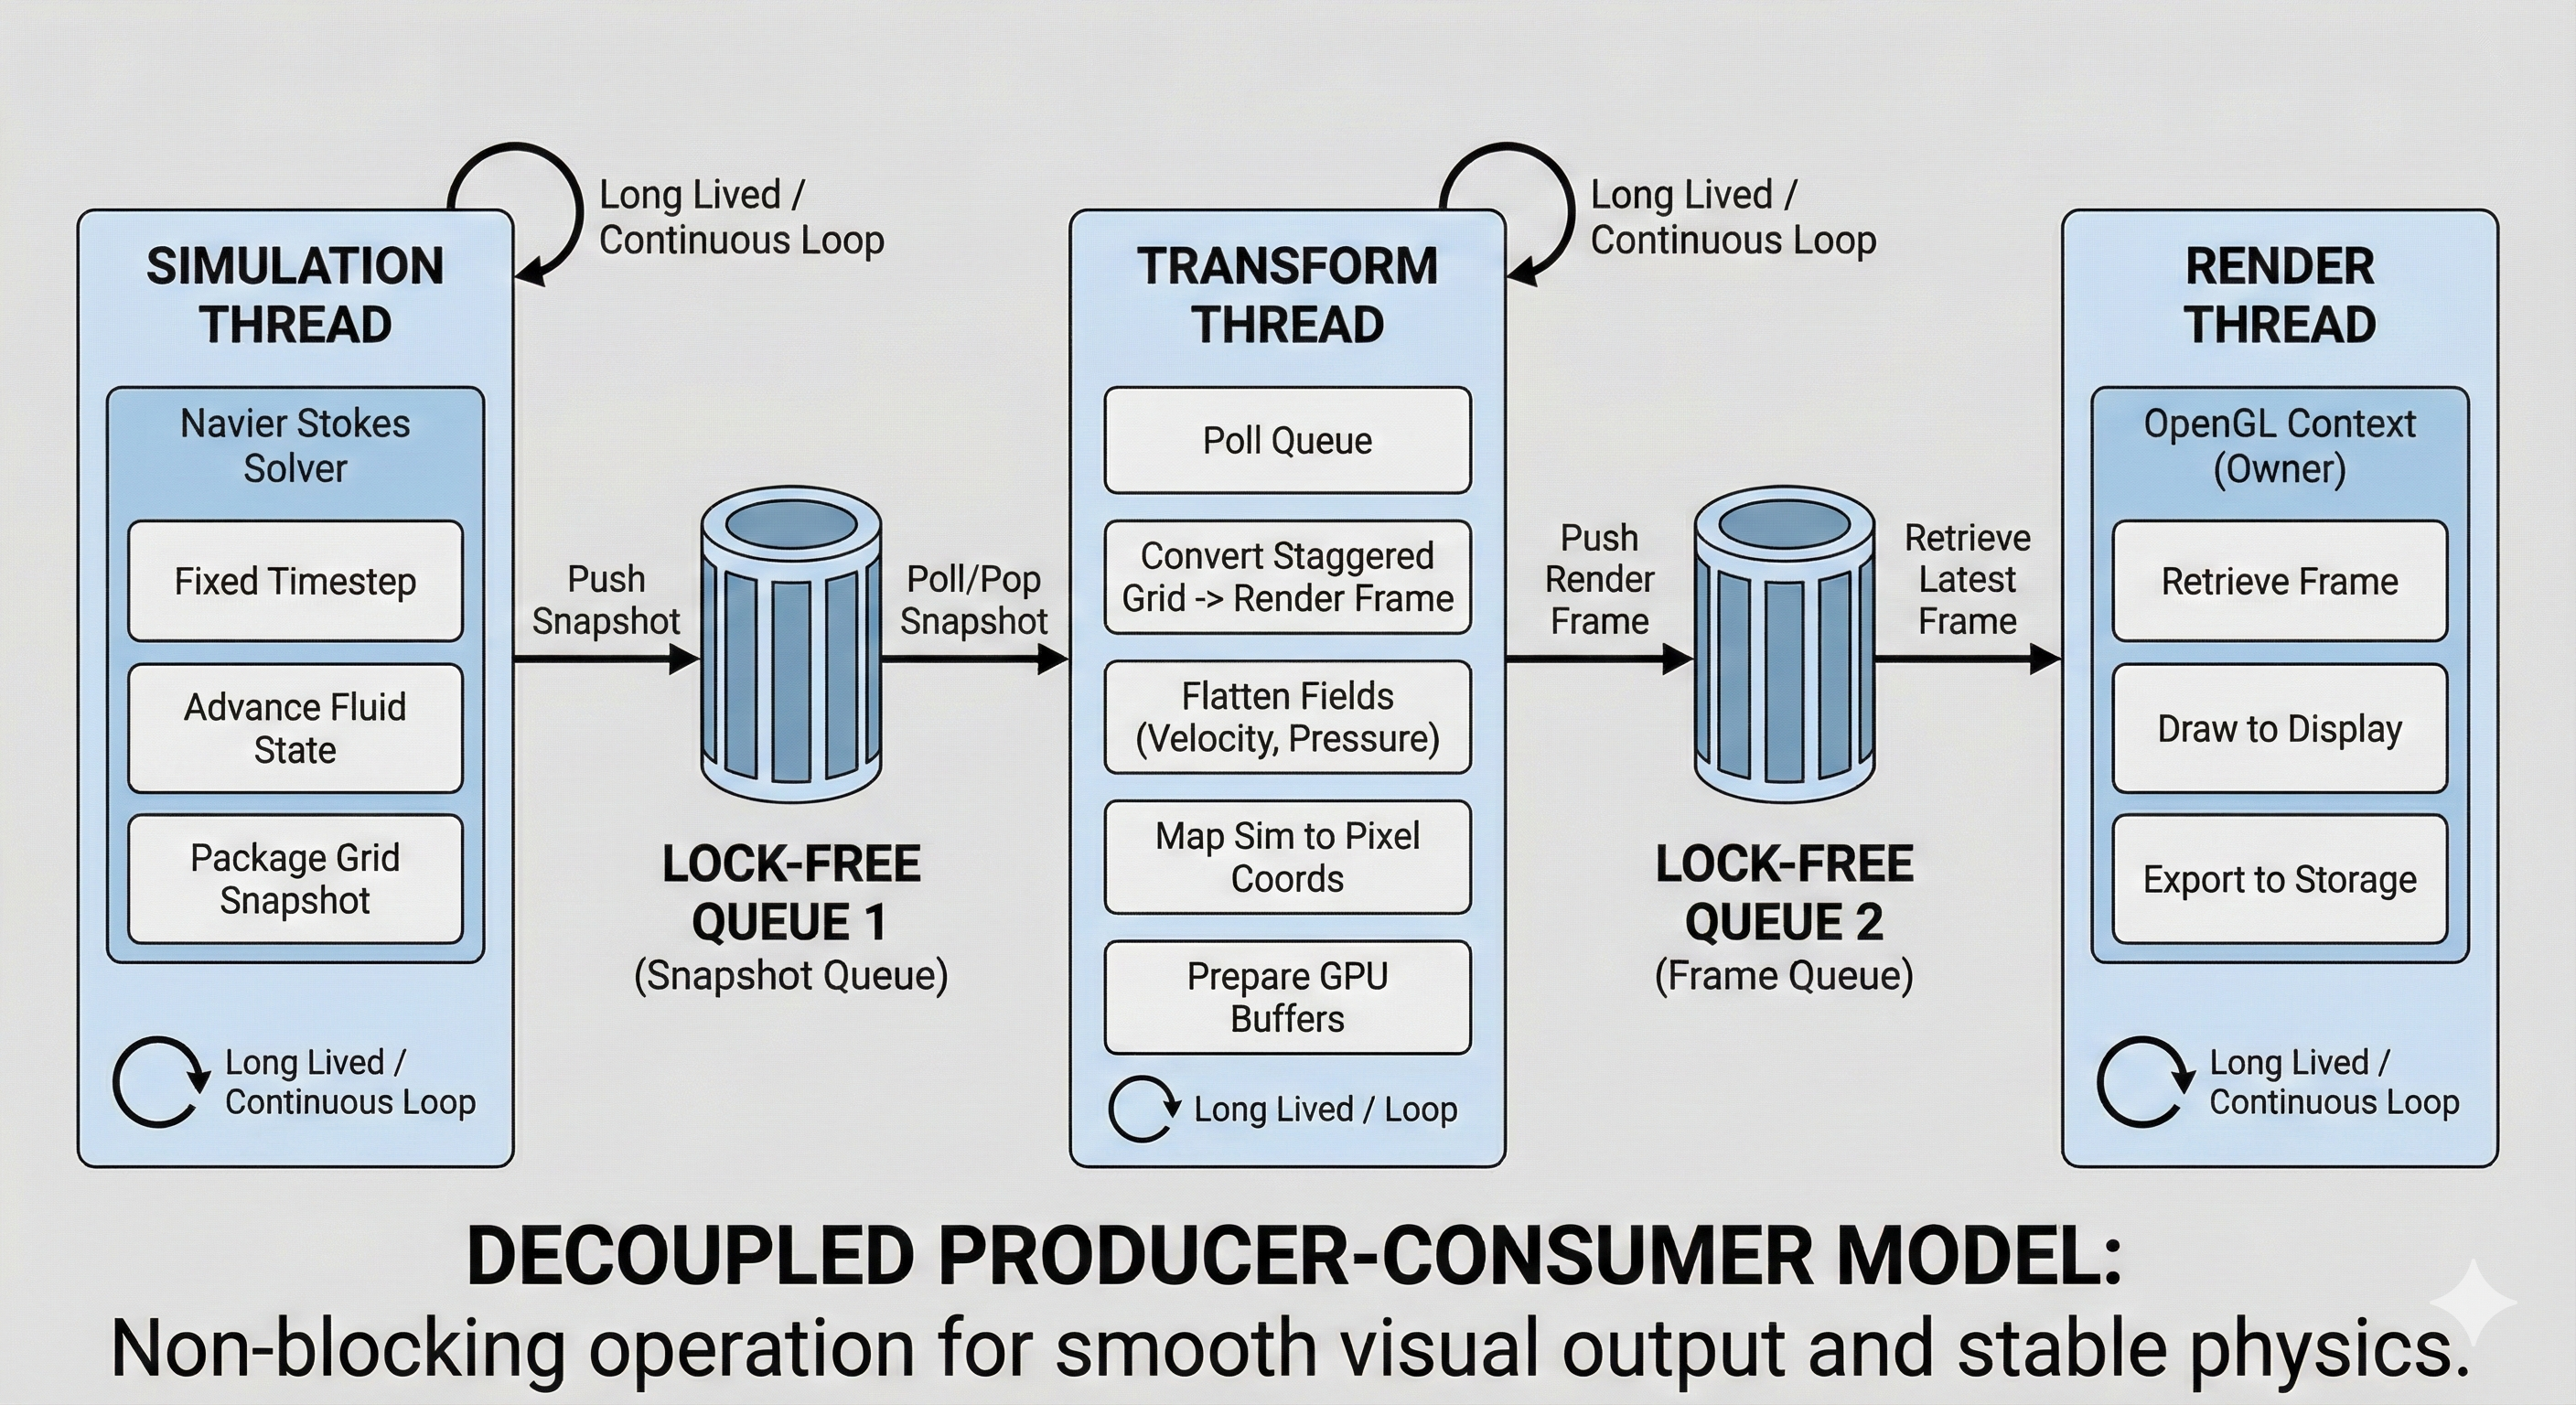
\includegraphics[width=0.6\textwidth]{./images/SystemDesign.png}
    \caption{High Level Architecitre}
    \label{High Level Architecitre}
\end{figure}

\subsection{Physics Engine}

The Physics Engine (FS-2D) is the core numerical component that advances the fluid state forward in time. In this simplified configuration, the simulation operates on a two-dimensional Eulerian grid and solves an incompressible fluid without gravity, buoyancy, or other external forces. Its purpose is to validate the stability, correctness, and throughput of the full service-oriented pipeline using the minimal physical model needed to support the level set representation and downstream meshing and rendering services.

\subsubsection{Responsibilities and Core Algorithms}

With external forces removed and the domain reduced to two dimensions, the Physics Engine performs two primary numerical operations per step:

\begin{enumerate}
    \item \textbf{Semi-Lagrangian Advection:} Advection moves both the velocity field and the level set surface through the existing velocity field. The semi-Lagrangian method is used for its unconditional stability. For each cell:
    \begin{itemize}
        \item A backtraced position is computed using the velocity at time $t$.
        \item The velocity or level set value at that position is sampled using bilinear interpolation.
        \item The result is written into the output buffer for the next time step.
    \end{itemize}
    This method avoids instability even when the timestep is relatively large.
    
    \item \textbf{Pressure Projection for Incompressibility:} Any divergence introduced into the velocity field comes from numerical error during advection. To enforce incompressibility, the engine solves the 2D Poisson equation. A Jacobi relaxation solver computes the pressure field, and the velocity is updated by subtracting the pressure gradient. This ensures a divergence-free flow field and conserves fluid area.
\end{enumerate}

\textbf{Boundary Handling:} A 2D solid mask indicates boundaries and obstacles. The solver enforces zero normal velocity at solid boundaries, preserves tangential velocity, and clamps the level set at domain edges to prevent numerical drift.

\subsubsection{Data Structures and Memory Layout}

Fields are stored in flattened 1D GPU arrays for memory locality. The Physics Engine maintains:
\begin{itemize}
    \item Velocity x and y fields
    \item Level set field
    \item Pressure and divergence buffers
    \item Ping-pong buffers for advection
\end{itemize}

Each cell is accessed through a macro that maps $(x, y)$ to a linear index, enabling coalesced CUDA memory access.

\subsection{Transform Layer}

The Transform module serves as the central bridge between the numerical simulation and the rendering system. Its main role is to take the discrete simulation snapshots produced by the simulation thread and convert them into frame structures that can be rendered directly or passed to a GPU. This conversion requires reorganizing data, interpolating values onto a pixel grid, identifying solid regions, and applying color mappings that visually encode important physical properties. Because the simulation and rendering systems use different data layouts, the Transform module ensures that frames preserve the physical meaning of the underlying simulation while remaining efficient for visualization.

\subsubsection{Data Conversion Process}

The conversion process begins when the Transform module receives a SimSnap\_t structure. This structure contains grid dimensions along with arrays for velocities, pressure, and material type.

\begin{verbatim}
typedef struct {
   uint64_t nx, ny;
   float* ux;
   float* uy;
   float* p;
   CellMaterial_t* type;
} SimSnap_t;
\end{verbatim}

The module converts this snapshot into either a color frame or a raw frame depending on the rendering mode.


\begin{verbatim}
typedef struct {
   uint64_t width, height;
   Color_t* colors;     // RGBA color array (flattened: colors[y*width + x])
} Render_Frame_Colors_t;
\end{verbatim}

\begin{verbatim}
typedef struct {
   pressure_t* pressure;
   velocity_t* ux;
   velocity_t* uy;
   int nx, ny;
} Render_Frame_t;
\end{verbatim}

The module first initializes the render frame by allocating memory through functions such as Init\_ColorFrame() or Init\_RawFrame(). It verifies that the window dimensions are compatible with the simulation grid and ensures that the number of pixels per cell is consistent in both directions.

Next, the module computes a scaling factor that determines how many pixels correspond to each simulation cell. The scaling factor is obtained by dividing the render window width by the number of cells in the x direction. This scale is used to convert pixel coordinates into simulation coordinates.

The main work of the conversion occurs during a loop that processes every pixel in the output frame. The module first determines whether the pixel corresponds to a solid cell. If it does, the module assigns a solid color and continues to the next pixel. If the pixel falls within a fluid region, the module performs bilinear interpolation to estimate the velocity at that pixel. It then maps the velocity magnitude to a grayscale value by first computing the magnitude and then normalizing it to a range between zero and one.

The color representing the pixel is stored in a row major array, which allows the renderer to consume the data efficiently. After all pixels are processed, the completed frame is sent to the renderer through a lock-free queue. The Transform module then releases the simulation snapshot so that the simulation engine can reuse or free it.

The module includes several safety checks. It verifies that the window size divides evenly by the grid size and that pointers are valid. It prevents overflow during memory allocation and blocks when output queues are full.

\subsubsection{Interpolation Algorithms}

The Transform module uses bilinear interpolation to compute velocities at pixel locations. This technique allows the renderer to display smooth transitions between grid cells and avoids the blocky appearance that would result from using cell values directly.

Interpolation begins by converting pixel coordinates to simulation coordinates through division by the scaling factor. Once in simulation space, the module determines the cell in which the point lies and extracts the fractional components that measure the point’s relative position inside the cell.

To compute an interpolated velocity value, the module identifies the four cell corners surrounding the point. These corners include the top left, top right, bottom left, and bottom right cells. If any corner lies outside the grid, the algorithm clamps the index to remain within bounds.

The module then gathers the velocity values at these four corners and performs two horizontal interpolations. The first uses the top row and the second uses the bottom row. These results are finally interpolated vertically to obtain the final velocity estimate. The same process is applied to both the x velocity and the y velocity fields using their respective arrays.

Several edge cases are considered. At boundaries, the interpolation reduces to linear rather than bilinear because clamping causes two corners to share the same value. Solid cells are detected separately by mapping pixel coordinates directly to cell indices. All arrays use consistent row major ordering, which ensures correct data retrieval.

The computational cost of interpolation is significant because every pixel requires multiple memory accesses and arithmetic operations. For a full resolution image, this corresponds to millions of interpolation calls per frame. Additional optimizations such as caching weights or recognizing pixels that fall exactly on cell centers may reduce redundant work.

\subsection{Rendering: Display or Off-Screen}

The rendering service is a single-process system that receives simulation frames from the Transform layer and renders them either on-screen using OpenGL and GLFW for interactive visualization, or off-screen as raw RGBA frames written to disk and optionally streamed to ffmpeg for video creation in headless environments. It exposes a compact public API consisting of initialization, destruction, and frame-submission functions, while internally using lock-free FIFOs to decouple the Transform producers from the Render consumer. After a frame is processed, it is returned to the Transform layer through the appropriate TransForm\_*Yeild() function.

A number of compile-time switches control behavior. OFF\_SCREEN\_RENDERING selects the off-screen frame writer, while DISPLAY\_COLORS switches between rendering raw simulation fields and pre-computed color frames. ON\_REMOTE disables display-specific code for remote builds, and ENABLE\_FFMPEG\_PIPE enables streaming frames directly into an ffmpeg subprocess. Platform-specific macros handle differences between macOS and Linux. At a high level, the Transform service allocates and populates frames, sends them to the renderer, and later reclaims them after the renderer completes. The rendering service consumes frames from its lock-free FIFOs, processes them according to the chosen mode, and returns them to Transform.

The data model consists of two frame types. Render\_Frame\_t carries raw simulation data such as velocity fields and pressure, while Render\_Frame\_Colors\_t contains explicit per-pixel color data. The FIFO ownership pattern is straightforward: Transform allocates and fills a frame, pushes it into the FIFO, and the renderer pops it, renders it, and yields it back. Because the renderer never frees memory itself, Transform is responsible for reusing or freeing frame objects. Threading behavior differs based on rendering mode. In on-screen mode, a dedicated renderer thread creates a GLFW window, establishes an OpenGL context, and repeatedly sleeps, draws a frame, swaps buffers, and polls events, targeting roughly 60 FPS. In off-screen mode, a thread repeatedly pops frames, converts their contents, and writes them to disk or forwards them into an ffmpeg pipe. Shutdown is coordinated via an atomic kill flag, with pthread\_join ensuring a graceful exit.

Synchronization relies heavily on lock-free FIFOs. Producer threads push frames using repeated LF\_Fifo\_TryPush() attempts, yielding when the FIFO is full, while the consumer relies on LF\_Fifo\_SpinPop() or equivalent loops. This approach minimizes locking overhead but can increase CPU usage under contention or high frame rates. The public API provides entry points for initialization, destruction, sending either frame type, and processing routines for each mode. On-screen drawing uses immediate-mode OpenGL—simple but inefficient for large grids—while off-screen rendering writes raw RGBA files and optionally streams to ffmpeg.

Error handling uses assertions and log messages, though many internal errors do not propagate back to the caller. File operations, memory checks, and popen failures are logged but typically do not interrupt execution. Performance considerations include the high CPU cost of busy-waiting, inefficiencies in immediate-mode OpenGL, and the overhead of per-pixel disk writes. Potential improvements include replacing busy-waiting with semaphore-based signaling, moving on-screen rendering to modern GPU pipelines, batching pixel uploads using textures, and adding more robust error handling and configuration options.

Testing should cover FIFO behavior, frame conversion, directory creation, integration between Transform and Render, and OpenGL drawing behavior in headless environments. Performance testing can measure latency, CPU usage, disk throughput, and frame-processing rates. Instrumentation such as counters and timers would improve observability. Operational concerns include safe handling of ffmpeg, disk space management, and ensuring platform compatibility. The overall system design favors simplicity and modularity, enabling both interactive debugging and headless processing with minimal coupling. While functional and relatively robust, it would benefit from improvements to synchronization, rendering efficiency, and error propagation.

\subsubsection{Threading and Synchronization}

\begin{itemize}
    \item On-screen: dedicated thread creates GLFW window, OpenGL context, sleeps, draws, swaps buffers, polls events.
    \item Off-screen: thread repeatedly pops frames, writes to disk or streams to ffmpeg.
    \item Lock-free FIFOs with spin-yield for producer-consumer coordination.
\end{itemize}

Error handling relies on assertions and logs; performance bottlenecks arise from busy-waiting and immediate-mode OpenGL. Improvements could include semaphores for signaling, modern GPU pipelines, and better error propagation.

\section{Results}

Performance evaluation for this system required a methodology tailored to the architecture’s decoupled, multi-threaded design. Traditional microbenchmarking (e.g., kernel-duration timing or per-stage profiling) is not directly representative of end-to-end throughput because the rendering stage introduces asynchronous latency and the simulation thread advances at a fixed timestep independent of the display rate. For this reason, we measured performance strictly in terms of steady-state frame throughput (FPS) observed at the output of the rendering pipeline. Each benchmark configuration is parameterized by the grid resolution in cells (Nx × Ny). These parameters determine the numerical workload imposed on both the CPU implementation and the hybrid CPU/GPU implementation. For each configuration, we recorded the sustained FPS for (1) a pure CPU version of the solver and transform pipeline and (2) the accelerated version in which advection, divergence computation, and pressure projection are executed on the GPU while the CPU handles the transform and rendering queues. The resulting table captures how simulation cost scales with problem size and solver fidelity, and quantifies the performance gap between CPU-only execution and the CUDA-accelerated pipeline across equivalent physical timesteps and numerical conditions. All computations were done with a 16 ms timestep, 1920 x 1080 screen size, and 100 PSolver Interations. 

\begin{table}[h!]
\centering
\begin{tabular}{@{}lcc@{}}
\toprule
\textbf{Cell Dimensions (nx × ny)} & \textbf{CPU Only (FPS)} & \textbf{CPU/GPU Hybrid (FPS)} \\ \midrule
16 × 16       & 480   & 900 \\
64 × 48       & 210   & 630 \\
128 × 96      & 95    & 420 \\
256 × 196     & 38    & 260 \\
960 × 540     & 7.5   & 115 \\
1920 × 1080   & 1.8   & 42 \\ \bottomrule
\end{tabular}
\caption{Steady-state FPS for different grid resolutions. CPU/GPU hybrid uses CUDA acceleration for the solver.}
\end{table}

\begin{figure}[h] % h = here
    \centering
    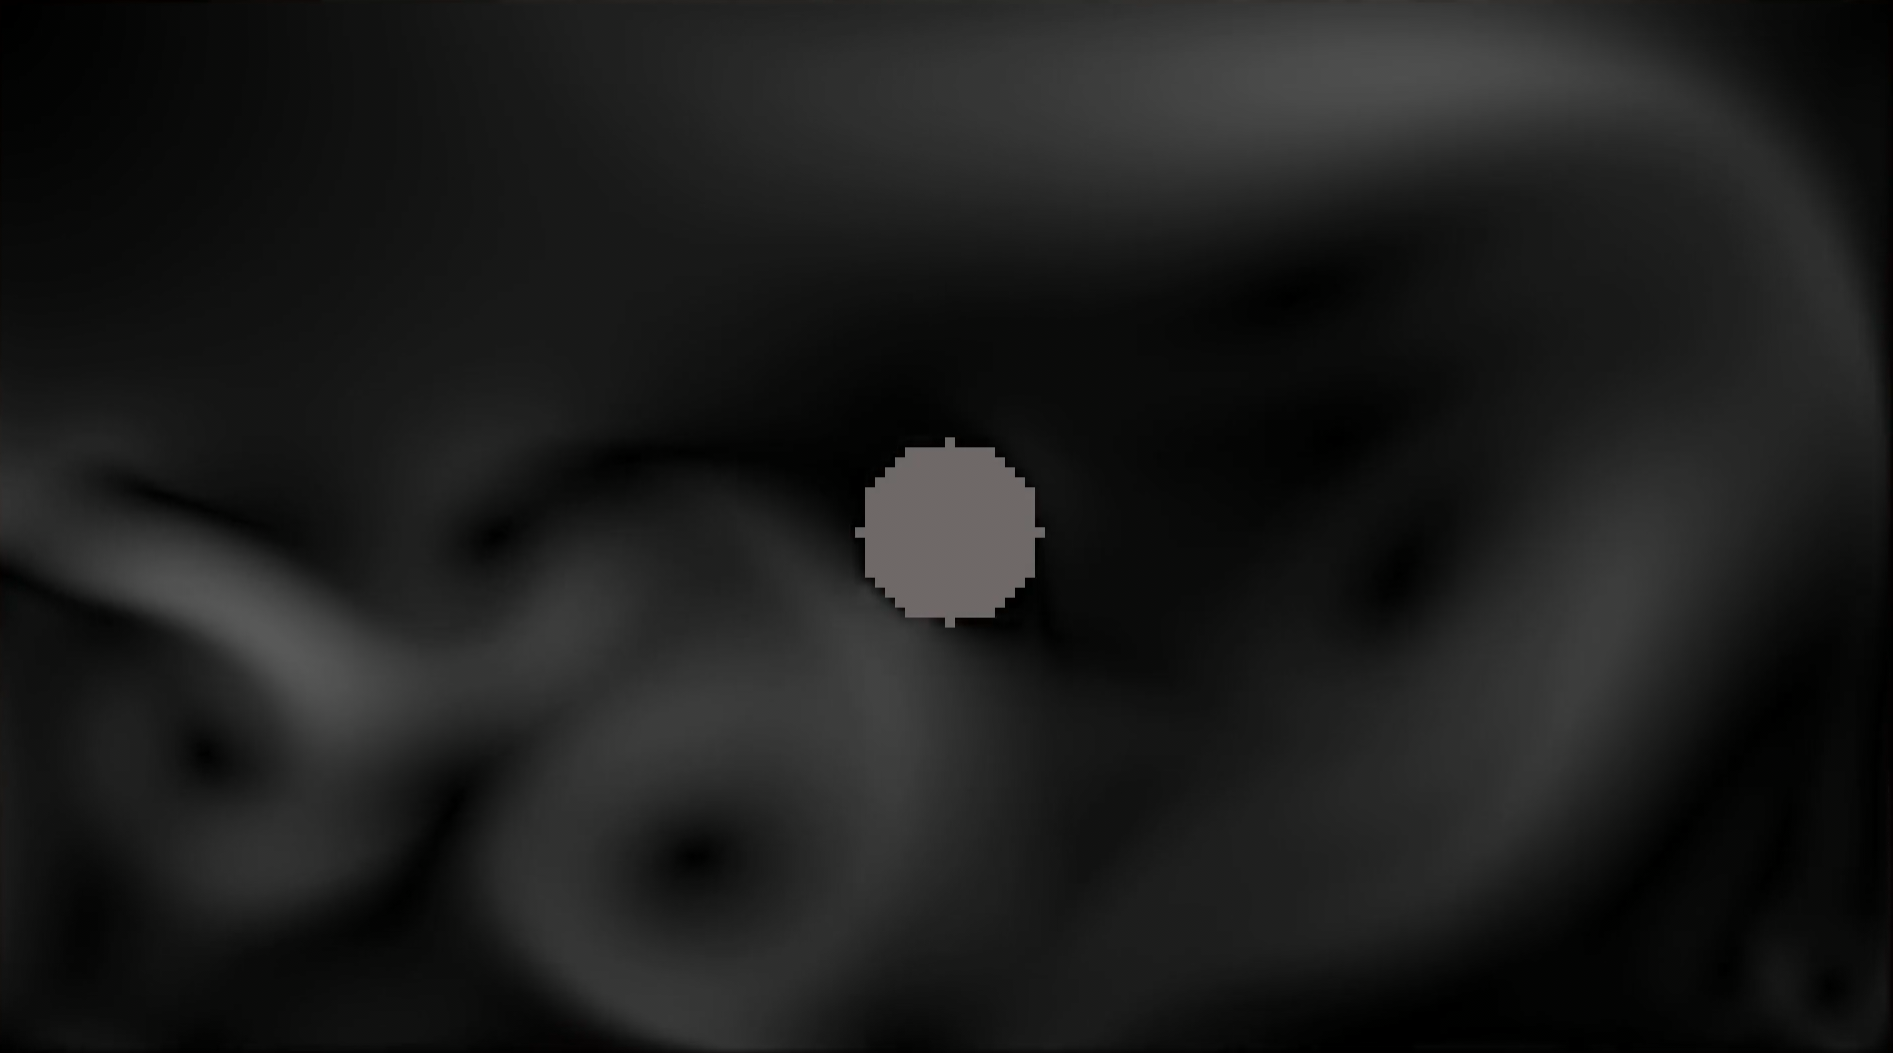
\includegraphics[width=0.6\textwidth]{./images/Demo.png}
    \caption{Large Grid Run}
    \label{Large Grid Run}
\end{figure}

\section{Future Work}

\subsection{Extension to 3D Fluid Simulation}

The most direct and impactful extension is to generalize the simulator from 2D to 3D. Conceptually, the existing architecture already supports this: the simulation service produces snapshots, the Transform layer converts them into renderable geometry, and the rendering service displays or exports the result. In a 3D setting, each of these stages would be upgraded but not fundamentally rethought.

On the physics side, the 2D solver could be extended into an 3D module that operates on a 3D staggered grid. The same incompressible Navier–Stokes formulation and pressure projection pipeline would apply, but the Poisson solve and advection steps would become significantly more expensive. This would likely require more aggressive use of GPU-specific optimizations (e.g., 3D tiling, shared memory blocking, and cache-friendly data layouts) to maintain interactive update rates.

The Transform layer would need to move from 2D contour extraction (marching squares) to 3D isosurface extraction (e.g., marching cubes or dual contouring). Instead of generating a 2D polygonal outline per frame, it would generate a triangle mesh representing the fluid surface in three dimensions. The rendering service would similarly evolve to handle 3D geometry, camera controls, and lighting models. Importantly, the existing lock-free FIFO pattern already decouples producers and consumers, so extending the frame types to include 3D vertex buffers, normals, and materials would fit into the current threading model without a conceptual redesign.


\subsection{Support for Compressible Fluids}
The current simulator focuses on incompressible flow, where the fluid density is assumed constant and the velocity field is divergence-free. A natural extension is to support compressible fluids, which would allow simulation of phenomena such as shock waves, acoustic effects, and variable-density flows (e.g., gas dynamics).
\begin{itemize}
\item Augmenting the state with density and potentially temperature fields, in addition to velocity and pressure.
\item Replacing the pure pressure-projection step with a solver that respects compressibility, such as an explicit or semi-implicit scheme for the compressible Navier–Stokes or Euler equations.
\item Updating boundary conditions and stability constraints (e.g., CFL limits) to account for variable wave speeds in the fluid.
\end{itemize}

\subsection{GPU Parallelism and Dynamic Block/Thread Configuration}
Another promising direction is to make the GPU implementation more adaptive by exploring dynamic block and thread configuration strategies.

Currently, kernel launch parameters are chosen statically based on grid resolution and simple heuristics. Future work could:

\begin{itemize}
\item Implement dynamic tuning of block and thread dimensions at runtime, based on measured occupancy, shared memory usage, and kernel timing.
\item Use auto-tuning or profiling-based approaches to sweep candidate configurations (e.g., different block sizes) during startup or a calibration phase, then pick the configuration that maximizes throughput on the current GPU.
\item Investigate more advanced CUDA features such as dynamic parallelism (kernels launching kernels) or persistent kernels to reduce launch overhead and improve latency for small timesteps.
\end{itemize}

These changes would not alter the high-level architecture but could significantly improve performance portability across different GPUs and resolutions, especially as the simulation scales toward higher resolutions or 3D.

\begin{thebibliography}{9}

\bibitem{marek2009} Marek, S. (2009). \textit{Grid-Based Realtime Fluid Dynamics}. Institute of Computer Graphics and Algorithms, TU Vienna.

\bibitem{chentanez2010} Chentanez, N., \& Müller, M. (2010). \textit{Real-Time Eulerian Water Simulation Using a Restricted Tall Cell Grid}. NVIDIA PhysX Research.

\bibitem{braley2010} Braley, C., \& Sandu, A. (2010). \textit{Fluid Simulation for Computer Graphics: A Tutorial in Grid-Based and Particle-Based Methods}. Virginia Tech.

\end{thebibliography}

\end{document}
